% !TEX root = Projektdokumentation.tex

Beim Mobile Quiz handelt es sich um eine Online Plattform für Computer und Smartphones. Auf dieser Plattform können Quizzes Erstellt und Durchgeführt werden. Mobile Quiz wird in verschiedenen HSR-Modulen (Computernetze, Informations- und Codierungstheorie, Informationssicherheit) und Weiterbildungskursen regelmässig eingesetzt. Mobile Quiz entstand 2012 aus einer Bachelorarbeit und wurde seither mehrmals erweitert. 

\bigskip
Die zu Beginn der Arbeit vorliegende Mobile Quiz Version umfasste zwar viele praktische Funktionen und Einstellungsmöglichkeiten, es mangelte aber an der Bedienbarkeit. Im Rahmen dieser Studienarbeit sollten deshalb einerseits die Benutzerfreundlichkeit erhöht und andererseits neue Funktionen hinzugefügt werden.

\bigskip

Mobile Quiz wird vor allem von Dozenten verwendet, um für Ihre Studenten Quizzes in Form von Lernhilfe während des Semesters zu bieten. Es besteht weiter die Möglichkeit die Quizzes entweder mit dem Typ Testatbedingung oder als Typ Prüfung zu erstellen und durchzuspielen. Die Wichtigsten Interaktionen mit dem Mobile Quiz System wurden in der folgenden Grafik festgehalten.
\begin{figure}[H]
	\centering
	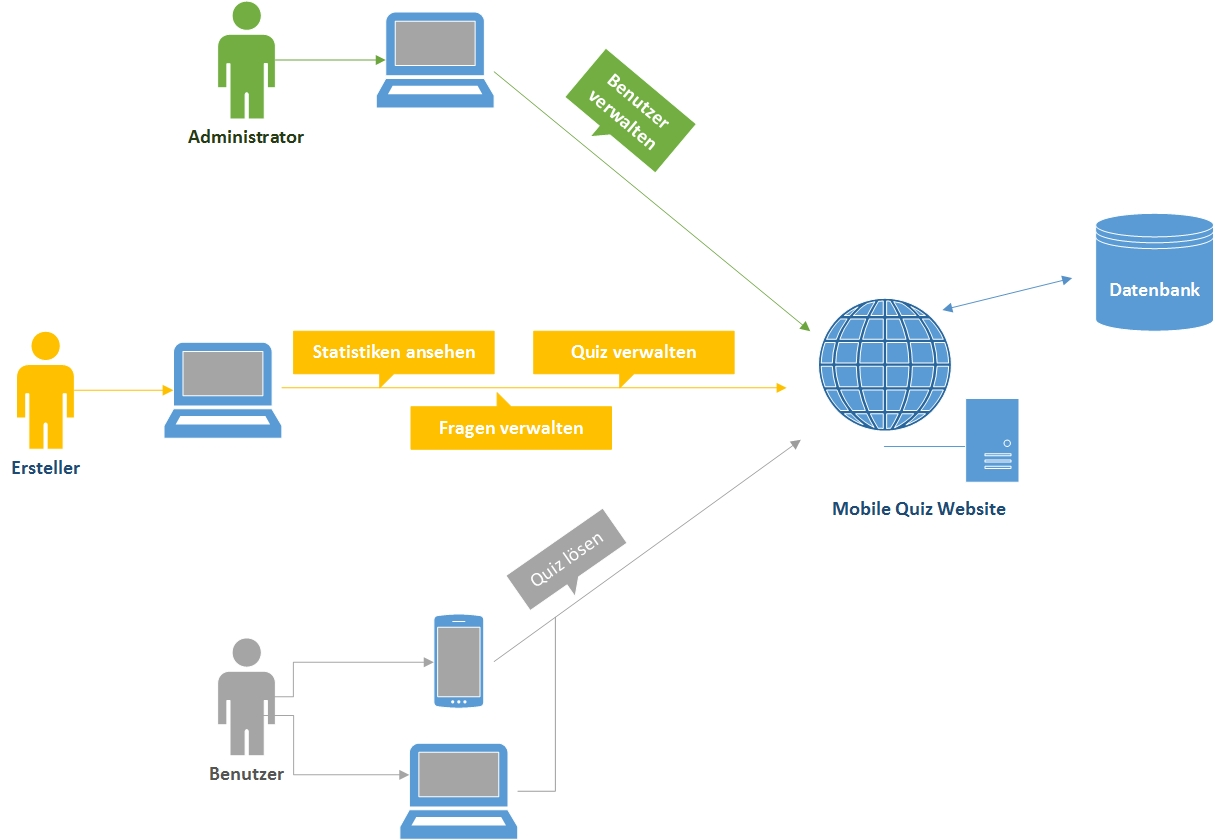
\includegraphics[width=1\textwidth]
	{Images/InteraktionMobileQuiz.jpg}
	\caption{Übersicht der wichtigsten Funktionen des Mobile Quiz}
\end{figure}

\bigskip

Das Vorgehen um sich in das Thema einzuarbeiten wurde wie folgt gewählt. In einem ersten Schritt wurde Mobile Quiz gründlich untersucht. Mit einem \gls{Usability-Test} wurden danach Optimierungsmöglichkeiten für Quizteilnehmer bestimmt. Anhand der Behebung der gefunden Fehlern aus der eigenen Untersuchung machte man sich mit dem Code und den eingesetzten Technologien vertraut. Im Rahmen einer Umfeldanalyse wurden ähnliche Online-Quiz Plattformen gesucht, getestet und bewertet. Die aus den vorgehenden Projektphasen gewonnenen Erkenntnisse halfen bei der Neugestaltung der Seiteninhalte sowie bei der Festlegung von neuen Funktionen. Beim Entwurf des Design wurden die anzuzeigenden Informationen bewusst auf das Nötigste beschränkt. Die Implementierung der Desings und Konzepte erfolgte während fünf Wochen. Da es sich bei dieser Arbeit um eine Erweiterung eines bestehenden Systems handelt, wurden die Technologien nicht neu gewählt. Es wurde die bereits bestehende Lösung mit PHP und JQuery für die Logik, der MySQL Datenbank für das Speichern der Daten und HTML zusammen mit CSS für die Darstellung verwendet. Nach der Implementierungsphase wurde die Arbeit mit einem \gls{Usability-Test} abgeschlossen.

\bigskip

Als Ergebnis dieser Arbeit konnte eine sowohl für den Quiz-Ersteller wie auch für den Teilnehmer wesentlich verbesserte Bedienbarkeit erreicht werden. Die Schritt-für-Schritt Benutzerführung erleichtert die Erstellung von Quiz, Fragen und Durchführungen. Dank der neuen Excel-Import Funktion lassen sich Quiz und Fragen einfacher erstellen. Durch die Erweiterung \glqq Fragen mit Bildern\grqq sind attraktivere Fragestellungen möglich. Die Konzeptänderung, welche pro Quiz mehrere Durchführungen möglich macht, erleichtert den Einsatz von Mobile Quiz im Unterricht mit mehreren Übungsgruppen. Dank dem neuen Design sollten sich die Quizteilnehmer schneller zurechtfinden. Dies belegt der Vergleich der Ergebnisse der beiden \gls{Usability-Test}s vor und nach der Überarbeitung des Mobile Quiz. Die jetzt vorliegende Mobile Quiz Version wird ab dem nächsten Semester produktiv eingesetzt. Die Umsetzung der in der Analysephase ausgearbeiteten statistischen Auswertungen könnte im Rahmen einer weiteren Studienarbeit erfolgen.